%% UTFPRCT-TEX, v1.0.6 wmeira on 2021/10/11
%% Copyright (C) 2020- by William H. T. Meira
%%
%% Modified version of project 'utfprpgtex' maintained 
%% by Luiz E. M. Lima
%%
%% This work may be distributed and/or modified under the
%% conditions of the LaTeX Project Public License, either version 1.3
%% of this license or (at your option) any later version.
%% The latest version of this license is in 
%%   http://www.latex-project.org/lppl.txt
%% and version 1.3 or later is part of all distributions of LaTeX
%% version 2005/12/01 or later.
%%
%% This work has the LPPL maintenance status `maintained'.
%%
%% The Current Maintainer of this work is William H. T. Meira.
%%
%% This project consists mainly of files: 'utfprct.cls', 'utfprct.tex', 
%% 'utfprct-dados.tex' 
%% 
%% The 'abntex2-alf.bst' and 'abntex2-num.bst' files are slightly
%% modified versions of the bibtex styles from abntex2 (v.1.9.7)
%% package to suit NBR6023/2018 (not yet implemented there). 
%% Complementary, 'abntex2-alf-en.bst' and 'abntex2-num-en.bst' are
%% english versions of the respective bibtex styles.
%%
%% Contribute to improve this project (github repo):
%% https://github.com/wmeira/utfprct-tex

%% Formato digital (sem folhas em branco): 
%% 'pretextualoneside': impressão dos elementos pré-textuais começa em qualquer lado da folha (anverso ou verso)
%% 'oneside': impressão dos elementos textuais e pós-textuais no anverso da folha (sem folhas em branco para o verso)

%% Formato impresso:
%% 'pretextualtwoside': impressão dos elementos pré-textuais começa sempre no anverso
%% 'oneside' ou 'twoside': impressão dos elementos textuais e pós-textuais `oneside` (anverso) ou `twoside` (anverso e verso, se mais de 100 páginas)

%% [Note] As legendas devem ser colocadas em cima do elemento (figura, tabela, quadro, algoritmo...) e os  \caption antes de entrar no ambiente. Obrigatoriamente, \fonte deve ser embaixo da elemento. Se for de criação do próprio autor, colocar "Autoria Própria." (Own Authorship.)
%\begin{figure}[htb]%% Ambiente figure
%\caption{Exemplo de caption}%% Legenda
%\label{fig:figura1}%% Rótulo
%\includegraphics[width=\textwidth]{./CapituloExemplo/figura1}%% Dimensões e localização
%\fonte{\citet{Larsson2003}.}%% Fonte (quando criado pelo autor, usar Autoria Própria)
%\end{figure}

%% Classe e opções de documento
\documentclass[%% Opções
%% -- Opções da classe MEMOIR --
  12pt,%% Tamanho da fonte: 10pt, 11pt, 12pt, etc.
  a4paper,%% Tamanho do papel: a4paper (A4), letterpaper (carta), etc.
  % fleqn,%% Alinhamento das equações à esquerda (comente para alinhamento centralizado)
  % leqno,%% Numeração das equações no lado esquerdo (comente para lado direito)
  oneside,%% IMPRESSÃO dos elementos textuais e pós-textuais: oneside (apenas no anverso) ou twoside (anverso e verso, se mais de 100 p.) (insere páginas em branco).
%%  
%% -- Opções da classe ABNTEX2 --
  sumario = abnt-6027-2012,%% Formatação do sumário: tradicional (estilo tradicional) ou abnt-6027-2012 (norma ABNT 6027-2012)
  chapter = TITLE,%% Títulos de capítulos em maiúsculas (comente para desabilitar)
  section = TITLE,%% Títulos de seções secundárias em maiúsculas (comente para desabilitar)
  % subsection = TITLE,%% Títulos de seções terciárias em maiúsculas (comente para desabilitar)
  % subsubsection = TITLE,%% Títulos de seções quartenárias em maiúsculas (comente para desabilitar)
%%  
%% -- Opções da classe UTFPRCT-TEX --
  pretextualoneside,%% Impressão dos elementos pré-textuais: pretextualoneside (anverso) ou pretextualtwoside (anverso e verso)
  fontetimes,%% Fonte do texto: fontetimes (times), fontearial (arial) ou fontecourier (courier), fontemodern (lmodern - default latex). Times and Arial are ABNT recommended
   %vinculoscoloridos,%% Cores nos vínculos (citações, arquivos, links, url, etc.) (comente para desabilitar). NBR 14724/2011: cor preta (inclusive hyperlinks)
  semrecuonosumario,%% Remoção do recuo dos itens no sumário (comente para adição do recuo, se estilo tradicional)
  %inserirbackref,%% Inserir backref na lista de referências (e.g., Citado na página...)
  usemakeindex,%% Compilação de glossários e índices utilizando makeindex (comente para desabilitar)
  legendascentralizadas,%% Alinhamento das legendas centralizado (comente para alinhamento à esquerda)
%%  
%% -- Opções da folha de aprovação -- 
%% O mais comum é anexar o PDF do termo de aprovação sem assinaturas. As opções abaixo são para o formato da pós-graduação UTFPR-PG (Ponta Grossa) e podem servir de placeholder para este template.
  %aprovacaoestiloppg,%% Folha de aprovação do programa de pós-graduação no estilo do PPG (comente para estilo padrão)
  %pardeassinaturas,%% Assinaturas na folha de aprovação em até duas colunas (comente para em uma única coluna)
  % linhasdeassinaturas,%% Linhas de assinaturas na folha de aprovação (comente para remover as linhas)
%%  
%% -- Opções do pacote babel (hifenização) -- % 
  %french,%% Idioma adicional para hifenização (suporte parcial)
  %spanish,%% Idioma adicional para hifenização (suporte parcial)
  english,%% Idioma adicional para hifenização  (colocar em último para doc. em inglês)  
  brazil%% Idioma principal do documento (último da lista) 
]{utfprct}%% Classe utfprct

%%%%%%%%
% Documento em Inglês: colocar o "english" como último idioma carregado no documentclass, sendo o último a língua principal do documento.
%%%%%%%%

%%%%%%%%
%% Configuração dos avisos (warnings)
%% Comportamento do Tex quando um PDF é incluído e possui uma versão mais nova que a versão mínima especificada em \pdfminorversion. Opções: -1 (no info), 0 (default, warning), 1 (error)
\pdfinclusionerrorlevel=-1%no warning 
%\pdfminorversion=5%pdf minor output version (default 5)

%% [Badbox] Underfull e Overfull nível de aviso (filtra o que está abaixo)
\hbadness=5000%0 até 10000 (max) nível de badness
\vbadness=1000%0 até 10000 (max) nível de badness
%\hfuzz=0.01pt%excesso permitido de largura (\hbox)para ser considerado overfull
%\vfuzz=0.001pt%excesso permitido de altura (\vbox) para ser considerado overfull
%\overfullrule=10mm%adicionar aviso visual para um badbox
%%%%%%%%

%%%%%%%%
%% Pacotes carregados nas classes:
%%   memoir: abstract, appendix, array, booktabs, ccaption, chngcntr, chngpage, dcolumn, delarray, enumerate, epigraph, framed, ifmtarg, ifpdf, index, makeidx, moreverb, needspace, newfile, nextpage, parskip, patchcmd, setspace, shortvrb, showidx, tabularx, titleref, titling, tocbibind, tocloft, verbatim, verse.
%%   memoir (similares): crop, fancyhdr, geometry, sidecap, subfigure, titlesec.
%%   abntex2: babel, bookmark, calc, enumitem, ifthen, hyperref, textcase.
%%   utfprct: abntex2cite, ae, algorithmic, amsmath, backref, breakurl, caption, subcaption, cmap, color, eepic, epic, epsfig, etoolbox, fancyhdr, fix-cm, fontenc, glossaries, graphics, graphicx, helvet, hyphenat, indentfirst, inputenc, lastpage, morewrites, nomencl, sfmath, sistyle, substr, times, xtab, pdfpages.

%% Pacotes adicionais (\usepackage[options]{package})
\usepackage{bigdelim, booktabs, colortbl, longtable, multirow}%% Ferramentas para tabelas
\usepackage{amssymb, amstext, amsthm, icomma}%% Ferramentas para linguagem matemática
\usepackage{pifont, textcomp, wasysym}%% Símbolos de texto
\usepackage{graphicx}
\usepackage{float}

% Refinamento tipográfico: diminui badboxes
\usepackage{microtype}%

%% Comandos personalizados (\newcommand{name}[num]{definition})
\newcommand{\cpp}{\texttt{C$++$}}%% C++
\newcommand{\latex}{\LaTeX}%% LaTeX
\newcommand{\ds}{\displaystyle}%% Tamanho normal das equações
\newcommand{\bsym}[1]{\boldsymbol{#1}}%% Texto no modo matemático em negrito
\newcommand{\mr}[1]{\mathrm{#1}}%% Texto no modo matemático normal (não itálico)
\newcommand{\der}{\mr{d}}%% Operador diferencial
\newcommand{\deri}[2]{\frac{\der#1}{\der#2}}%% Derivada ordinária
\newcommand{\derip}[2]{\frac{\partial#1}{\partial#2}}%% Derivada parcial
\newcommand{\pare}[1]{\left(#1\right)}%% Parênteses
\newcommand{\colc}[1]{\left[#1\right]}%% Colchetes
\newcommand{\chav}[1]{\left\lbrace#1\right\rbrace}%% Chaves
\newcommand{\sen}{\operatorname{sen}}%% Operador seno
\newcommand{\senh}{\operatorname{senh}}%% Operador seno hiperbólico
\newcommand{\tg}{\operatorname{tg}}%% Operador tangente
\newcommand{\tgh}{\operatorname{tgh}}%% Operador tangente hiperbólico  
\ifthenelse{\equal{\languagename}{english}}{%%
\newcommand{\nomeequacao}{Equation}
\newcommand{\nomeequacoes}{Equations}
}{%default pt
\newcommand{\nomeequacao}{Equação}
\newcommand{\nomeequacoes}{Equações}
}%  
\newcommand{\seqref}[1]{\nomeequacao~\eqref{#1}}%% Referência de uma única equação
\newcommand{\meqref}[1]{\nomeequacoes~\eqref{#1}}%% Referência de multiplas equações
\newcommand{\citep}[1]{\cite{#1}}%% Atalho para citação implícita
\newcommand{\citet}[1]{\citeonline{#1}}%% Atalho para citação explícita
\newcommand{\citepa}[1]{(\citeauthor{#1})}%% Atalho para citação implícita (somente autor)
\newcommand{\citeta}[1]{\citeauthoronline{#1}}%% Atalho para citação explícita (somente autor)
\newcommand{\citepy}[1]{(\citeyear{#1})}%% Atalho para citação implícita (somente ano)
\newcommand{\citety}[1]{\citeyear{#1}}%% Atalho para citação explícita (somente ano)

%allow fixed size on collums with text position
\newcolumntype{L}[1]{>{\raggedright\let\newline\\\arraybackslash\hspace{0pt}}m{#1}}
\newcolumntype{C}[1]{>{\centering\let\newline\\\arraybackslash\hspace{0pt}}m{#1}}
\newcolumntype{R}[1]{>{\raggedleft\let\newline\\\arraybackslash\hspace{0pt}}m{#1}}

%%%%%%%%%%%%%%%%%%%%%%%%%%%%%%%%%%%%%%%%%%%%%%%
%%%%%%%%%%%%%%%%%%%%%%%%%%%%%%%%%%%%%%%%%%%%%%%
%% Configuração das entradas
%%

%% Arquivo de dados do modelo de documento LaTeX para produção de trabalhos acadêmicos da UTFPR
%% UTFPRCT-TEX, v1.0.6 wmeira on 2021/10/11
%% Copyright (C) 2020- by William H. T. Meira
%%
%% Modified version of project 'utfprpgtex' maintained 
%% by Luiz E. M. Lima
%%
%% This work may be distributed and/or modified under the
%% conditions of the LaTeX Project Public License, either version 1.3
%% of this license or (at your option) any later version.
%% The latest version of this license is in
%%   http://www.latex-project.org/lppl.txt
%% and version 1.3 or later is part of all distributions of LaTeX
%% version 2005/12/01 or later.
%%
%% This work has the LPPL maintenance status `maintained'.
%%
%% The Current Maintainer of this work is William H. T. Meira.
%%
%% This project consists mainly of files: 'utfprct.cls', 'utfprct.tex', 
%% 'utfprct-dados.tex' 
%% 
%% The 'abntex2-alf.bst' and 'abntex2-num.bst' files are slightly
%% modified versions of the bibtex styles from abntex2 (v.1.9.7)
%% package to suit NBR6023/2018 (not yet implemented there). 
%% Complementary, 'abntex2-alf-en.bst' and 'abntex2-num-en.bst' are
%% english versions of the respective bibtex styles.
%%
%% Contribute to improve this project (github repo):
%% https://github.com/wmeira/utfprct-tex

%%%%%%%%%%%%%%%%%%%%%%%%%%%%%%%%%%%%%%%%%%%%%%%
%%%%%%%%%%%%%%%%%%%%%%%%%%%%%%%%%%%%%%%%%%%%%%%
%% Tutorial do Documento de Dados 
%%%%%%%%%%%%%%%%%%%%%%%%%%%%%%%%%%%%%%%%%%%%%%%
%%
%% O 'utfprct-dados.tex' contém todos as informações do documento, 
%% metadados e outros valores importantes para o preenchimento dos 
%% elementos pré-textuais: capa, folha de rosto, resumo, abstract.
%% 
%% Não é necessário preencher todos os campos, existem campos mais
%% específicos para o tipo de documento sendo elaborado. Quando TCC,
%% por exemplo, não é necessário definir dados do programa de 
%% pós-graduação. Todos os dados inseridos estarão disponíveis para
%% inserção no tex usando o padrão '\imprimir + nomedodadominusculo'. 
%% Por exemplo, para imprimir o tipo do documento ('\TipoDeDocumento'),
%% usar '\imprimirtipodedocumento'.
%%
%% É possível customizar a descrição do documento na folha de rosto. 
%% Exemplos de descrição são fornecidos para guiar a escrita do texto,
%% em que pode-se utilizar os dados já definidos com o padrão descrito.
%%
%% Existe a possibilidade de inserir dados de uma instituição de 
%% cotutela quando se aplicar. 
%%
%% Os dados da ficha catalográfica são fornecidos pela biblioteca
%% e, na maioria das vezes, apenas anexa-se a folha digitalizada
%% na região definida dos elementos pré-textuais.
%%
%% A folha de aprovação é, na maioria das vezes, fornecido 
%% digitalmente pelo departamento ou pelo orientador após a defesa e 
%% deverá ser anexada ao documento na região definida dos elementos 
%% pré-textuais. Recomenda-se apenas anexar a folha de aprovação sem
%% precisar alterar os dados específicos aqui presentes, pois foram
%% criados originalmente para o template da folha de aprovação da
%% UTFPR-PG, presente no projeto base, e foram apenas mantidos.
%%
%%%%%%%%%%%%%%%%%%%%%%%%%%%%%%%%%%%%%%%%%%%%%%%
%%%%%%%%%%%%%%%%%%%%%%%%%%%%%%%%%%%%%%%%%%%%%%%

%%%%%%%%%%%%%%%%%%%%%%%%%%%%%%%%%%%%%%%%%%%%%%%
%% Informações do Documento
%%%%%%%%%%%%%%%%%%%%%%%%%%%%%%%%%%%%%%%%%%%%%%%

%% Tipo de documento (opções: "Tese", "Dissertação", "Trabalho de Conclusão de Curso"
\TipoDeDocumento{Oficina de integração 1 - Relatório Final}%copiar exatamente uma das opções 

%% [abstract] Document type: "Thesis", "Dissertation", "Bachelor Thesis"
%\DocumentType{Thesis}%

%% Nível de formação: "Doutorado", "Mestrado", "Bacharelado"
%\NivelDeFormacao{Doutorado}%

%% [abstract] Formation level: "Doctorate", "PhD", "Master's Degree", "Bachelor's Degree"
%\FormationLevel{PhD}%

%% Título ou grau pretendido: "Doutor", "Mestre" ou "Bacharel"
%\TituloPretendido{Doutor}%

%%%%%%%%%%%%%%%%%%%%%%%%%
%% Por padrão, o título principal será o \TituloDoDocumento (português)
%% Se a língua do documento for definida como inglês, será o \DocumentTitle

%% Título do documento em PORTUGUÊS (resumo)
\TituloDoDocumento{%%
EEX21_Equipe5_Relatório_EstabilizadorDeDoisEixosParaCâmeras
}%


%% Título em múltiplas linhas na capa, folha de rosto e termo de aprovação
%% Use o comando \par para indicar a quebra de linha
%%
%% A CAPA apresentará o título no formato de múltiplas linhas
%% para a respectiva língua do documento definida.
%%
%% Na folha de rosto, caso a língua do documento não seja português, aparecerá o
%% \TituloEmMultiplasLinhasIngles seguido pela tradução \TituloEmMultiplasLinhas
%%
\TituloEmMultiplasLinhas{%%
Estabilizador de dois eixos para câmeras
}%

\TituloEmMultiplasLinhasIngles{%%
\par
}%

%%%%%%%%%%%%%%%%%%%%%%%%%


%% Data da defesa
%\Dia{1}%% Dia (opcional: usado na ficha catalográfica apenas)
%\MesPorExtenso{janeiro}%% mês por extenso (opcional: usado na ficha catalográfica apenas)
\Ano{2022}%% Ano

%% Palavras-chave e keywords (máximo 5)
\NumeroDePalavrasChave{5}%% Número de palavras-chave 
\PalavraChaveA{Estabilizador para câmeras}%% Palavra-chave A
\PalavraChaveB{Servo motores}%% Palavra-chave B
\PalavraChaveC{Suporte articulado}%% Palavra-chave C
\PalavraChaveD{Manipulação de dados com arduino}%% Palavra-chave D
%\PalavraChaveE{Palavra-chave E}%% Palavra-chave E

\NumeroDeKeywords{\imprimirnumerodepalavraschave}%% Número de keywords (mesmo que palavras-chave)
\KeywordA{Keyword A}%% Keyword A
\KeywordB{Keyword B}%% Keyword B
\KeywordC{Keyword C}%% Keyword C
\KeywordD{Keyword D}%% Keyword D
\KeywordE{Keyword E}%% Keyword E

%%%%%%%%%%%%%%%%%%%%%%%%%%%%%%%%%%%%%%%%%%%%%%%
%% Informação do Autor(a) ou Autores(as) (TCC)
%%%%%%%%%%%%%%%%%%%%%%%%%%%%%%%%%%%%%%%%%%%%%%%

%%% Autor(a)
%% Usado para citação: "\SobrenomeDoAutor, PrenomeDoAutor" (ex: "Doe, John" ou "Doe, J.")
\NomeDoAutor{Henrique Francisco Knapp}%% Nome completo do(a) autor(a)
%\SobrenomeDoAutor{Último Nome}%% Último nome do(a) autor(a)
%\PrenomeDoAutor{Nome do(a) Autor(a) Sem Último}%% Nome do(a) autor(a) sem último nome

%%% Autor(a) 2 (opcional)
%% *Considera apenas se "\TipoDeDocumento" == "Trabalho de Conclusão de Curso"
\AtribuiAutorDois{true}%% Insere ou remove autor(a) 2: "true" ou "false"
\NomeDoAutorDois{Fernando Henrique Ratusznei Caetano}%% Nome completo do(a) autor(a) 2
%\SobrenomeDoAutorDois{Último Nome}%% Último nome do(a) autor(a) 2
%\PrenomeDoAutorDois{Nome do(a) Autor(a) 2 Sem Último}%% Nome do(a) autor(a) 2 sem último nome

%%% Autor(a) 3 (opcional)
%% *Considera apenas se "\TipoDeDocumento" == "Trabalho de Conclusão de Curso"
\AtribuiAutorTres{true}%% Insere ou remove autor(a) 3: "true" ou "false"
\NomeDoAutorTres{Robson Borges Dos Santos}%% Nome completo do(a) autor(a) 3
%\SobrenomeDoAutorTres{Último Nome}%% Último nome do(a) autor(a) 3
%\PrenomeDoAutorTres{Nome do(a) Autor(a) 3 Sem Último}%% Nome do(a) autor(a) 3 sem último nome

%%%%%%%%%%%%%%%%%%%%%%%%%%%%%%%%%%%%%%%%%%%%%%%%%%
%% Informações do Orientador(a) e Coorientador(a)
%%%%%%%%%%%%%%%%%%%%%%%%%%%%%%%%%%%%%%%%%%%%%%%%%%

%% Orientador(a)
%% Usado para citação: "\SobrenomeDoOrientador, PrenomeDoOrientador" (ex: "Doe, John" ou "Doe, J.")
\AtribuicaoOrientador{Orientador(a)}%% Atribuição "Orientador(a)"
\TituloDoOrientador{Prof(a). Dr(a).}%% Título do(a) orientador(a)
\NomeDoOrientador{Nome Completo do(a) Orientador(a)}%% Nome completo do(a) orientador(a)
\SobrenomeDoOrienador{Último Nome}%% Último nome do(a) orientador(a)
\PrenomeDoOrientador{Nome do(a) Orientador(a) Sem Último}%% Nome do(a) orientador(a) sem último nome

%% Coorientador(a) (opcional)
%% Usado para citação: "\SobrenomeDoCoorientador, PrenomeDoCoorientador" (ex: "Doe, John" ou "Doe, J.")
\AtribuiCoorientador{true}%% Insere ou remove o(a) coorientador(a): "true" ou "false"
\AtribuicaoCoorientador{Coorientador(a)}%% Atribuição "Coorientador(a)"
\TituloDoCoorientador{Prof(a). Dr(a).}%% Título do(a) coorientador(a)
\NomeDoCoorientador{Nome Completo do(a) Coorientador(a)}%% Nome completo do(a) coorientador(a)
\SobrenomeDoCoorienador{Último Nome}%% Último nome do(a) coorientador(a)
\PrenomeDoCoorientador{Nome do(a) Coorientador(a) Sem Último}%% Nome do(a) coorientador(a) sem último nome

%%%%%%%%%%%%%%%%%%%%%%%%%%%%%%%%%%%%%%%%%%%%%%%%%%
%% Informações da Instituição
%%%%%%%%%%%%%%%%%%%%%%%%%%%%%%%%%%%%%%%%%%%%%%%%%%

%% Nome da instituição
\Instituicao{Universidade Tecnológica Federal do Paraná}

%% [abstract] Institution name (*nome sem traduzir é o recomendado para docs. da UTFPR)
%\Institution{Universidade Tecnológica Federal do Paraná}

%% Sigla da Instituição
\SiglaInstituicao{UTFPR}

%% Nome da cidade (câmpus)
\Cidade{Curitiba}

%% Diretoria: "Graduação e Educação Profissional" ou "Pesquisa e Pós-Graduação" (opcional)
%\Diretoria{Pesquisa e Pós-Graduação}

%% Nome do departamento ou da coordenação (opcional: mais comum no Bacharelado: Departamento de Informática)
\Departamento{Curso de Engenharia de Computação}

%% Sigla do departamento (opcional, ex: DAINF, DAMEC, DAMAT...)
%\SiglaDepartamento{DPT}

%% Nome do curso bachalerado ou pós-graduação (PPG) (ex: "Engenharia de Computação",  "Engenharia El{\'e}trica e Inform{\'a}tica Industrial") 
\Curso{Engenharia de Computação}


%% Programa ou nome do curso completo (capa)
%% "Bachalerado em Engenharia de Computação"
%% "Programa de Pós-Graduação em Engenharia Elétrica e Informática Industrial"
\Programa{Programa de Pós-Graduação em \imprimircurso}

%% Sigla do programa de pós-graduação (opcional, ex: CPGEI, PPGCA)
\SiglaDoPPG{PPG}

%% Nome da área de concentração
\AreaDeConcentracao{Nome da Área de Concentração}

%%%%%%%%%%%%%%%%%%%%%%%%%%%%%%%%%%%%%%%%%%%%%%%%%%%%%%
%% Informações de Cotutela (Duplo Grau) (opcional)
%%%%%%%%%%%%%%%%%%%%%%%%%%%%%%%%%%%%%%%%%%%%%%%%%%%%%%

%% Insere dados de cotutela: "true" ou "false"
\AtribuiCotutela{false}

%% Nome da instituição de cotutela
\InstituicaoCotutela{Universidade Da Cotutela}

%% [abstract] Institution name
\InstitutionCotutela{Double Degree University}

%% Sigla da instituição de cotutela
\SiglaInstituicaoCotutela{UC}

%% Nome do departamento ou da coordenação da inst. de cotutela (mais comum no Bacharelado: Departamento de Informática)
\DepartamentoCotutela{Nome do Departamento ou da Coordenação}

%% Sigla do departamento da inst. cotutela (ex: DAINF, DAMEC, DAMAT...)
\SiglaDepartamentoCotutela{DPT-EXT}

%% Nome do curso bachalerado ou pós-graduação (PPG) na instituição de cotutela (ex: "Engenharia de Computação",  "Engenharia El{\'e}trica e Inform{\'a}tica Industrial")
\CursoCotutela{Nome do Curso Cotutela}

%% [abstract] Course name 
\CourseCotutela{Second Degree Course}

%% Programa ou nome do curso completo na inst. cotutela (capa)
%% "Bachalerado em Engenharia de Computação"
%% "Programa de Pós-Graduação em Engenharia Elétrica e Informática Industrial"
\ProgramaCotutela{Programa de Doutoral em \imprimircursocotutela}

%% Sigla do programa externo de pós-graduação
\SiglaDoPPGCotutela{PPG-EXT}

%% Nome da área de concentração na instituição de cotutela
\AreaDeConcentracaoCotutela{Nome da Área de Concentração}

%% Nível de formação que será fornecido na referência do doc.
\NivelDeFormacaoResumo{Duplo doutorado}
\FormationLevelAbstract{Double PhD}

%% Informacoes do orientador(a) na instituição de cotutela

%% Orientador(a) da instituição de cotutela
%% Usado para citação: "\SobrenomeDoOrientador, PrenomeDoOrientador" (ex: "Doe, John" ou "Doe, J.")
\AtribuicaoOrientadorCotutela{Orientador(a)}%% Atribuição "Orientador(a)"
\TituloDoOrientadorCotutela{Prof(a). Dr(a).}%% Título do(a) orientador(a)
\NomeDoOrientadorCotutela{Nome Completo do(a) Orientador(a)}%% Nome completo do(a) orientador(a)
\SobrenomeDoOrienadorCotutela{Último Nome}%% Último nome do(a) orientador(a)
\PrenomeDoOrientadorCotutela{Nome do(a) Orientador(a) Sem Último}%% Nome do(a) orientador(a) sem último nome

%% Coorientador(a) da instituição de cotutela
%% Usado para citação: "\SobrenomeDoCoorientador, PrenomeDoCoorientador" (ex: "Doe, John" ou "Doe, J.")
\AtribuiCoorientadorCotutela{false}%% Insere ou remove o(a) coorientador(a) da cotutela: "true" ou "false"
\AtribuicaoCoorientadorCotutela{Coorientador(a)}%% Atribuição "Coorientador(a)"
\TituloDoCoorientadorCotutela{Prof(a). Dr(a).}%% Título do(a) coorientador(a)
\NomeDoCoorientadorCotutela{Nome Completo do(a) Coorientador(a)}%% Nome completo do(a) coorientador(a)
\SobrenomeDoCoorienadorCotutela{Último Nome}%% Último nome do(a) coorientador(a)
\PrenomeDoCoorientadorCotutela{Nome do(a) Coorientador(a) Sem Último}%% Nome do(a) coorientador(a) sem último nome

%%%%%%%%%%%%%%%%%%%%%%%%%%%%%%%%%%%%%%%%%%%%%%%%%%
%% Folha de Rosto
%%%%%%%%%%%%%%%%%%%%%%%%%%%%%%%%%%%%%%%%%%%%%%%%%%

%% Descrição do documento na folha de rosto (exemplos)
\DescricaoDoDocumento{
Relatório final do projeto desenvolvido na disciplina de Oficina de Integração 1, do curso de Engenharia de Computação, da
Universidade Tecnológica Federal do Paraná (UTFPR).\\
\\Orientadores:\\Prof. Juliano Mourão Vieira.\\Prof. Ronnier Frates Rohrich
}


%% Insere ou remove descrição da cotutela (extra) na folha de rosto: "true" ou "false". 
%% Se "true", a descrição do documento será colocada na folha de rosto, logo abaixo do orientador(a) e coorientador(a) da primeira inst. e depois o orientador(a) e coorientador(a) da inst. de cotutela. 
%% Se "false", os nomes do orientador(a) e coorientador(a) aparecerão logo abaixo do orientador(a) da primeira instituição, sem uma descrição extra. Neste caso, recomenda-se revisar a "\DescricaoDoDocumento" para contemplar ambas as instituições.   
\AtribuiDescricaoCotutela{false}

%% Segunda Descricao da Inst. de Cotutela na folha de rosto (exemplos)
\DescricaoDoDocumentoCotutela{
\imprimirtipodedocumento\ apresentado(a) como requisito à obtenção do título de \imprimirtitulopretendido\ em \imprimircursocotutela, do \imprimirppgoudepartamentocotutela, da \imprimirinstituicaocotutela.  
\imprimirtipodedocumento\ apresentada à Comissão de Acompanhamento de Tese do Programa Doutoral em \imprimircursocotutela\ do \imprimirinstituicaocotutela\ (\imprimirsiglainstituicaocotutela) como requisito à obtenção de grau de \imprimirtitulopretendido\ na área de concentração \imprimirareadeconcentracaocotutela.
}%% Realize as modificações pertinentes no arquivo "utfprct-dados.tex"

%% Ferramenta para criação de índices
\makeindex%% Não comente esta linha

%% Ferramenta para criação de glossários
\makeglossaries%% Não comente esta linha

%% Entradas da lista de abreviaturas, siglas e acrônimos
\include{./PreTexto/entradas-acronimos}% Comente para remover este item

%% Entradas do glossário
\include{./PosTexto/entradas-glossario}% Comente para remover este item

%% Ferramenta para criação de nomenclaturas
\makenomenclature%% Não comente esta linha

%%%%%%%%%%%%%%%%%%%%%%%%%%%%%%%%%%%%%%%%%%%%%%%
%%%%%%%%%%%%%%%%%%%%%%%%%%%%%%%%%%%%%%%%%%%%%%%
%% Início do documento
%%
\begin{document}%% Não comente esta linha

%%%%%%%%%%%%%%%%%%%%%%%%%%%%%%%%%%%%%%%%%%%%%%%
%%%%%%%%%%%%%%%%%%%%%%%%%%%%%%%%%%%%%%%%%%%%%%%
%% Formatação de páginas de elementos pré-textuais
%%
\pretextual%% Não comente esta linha


%%%%%%%%%%%%%%%%%%%%%%%%%%%%%%%%%%%%%%%%%%%%%%%
%% Capa
%%
\incluircapa%% Comente para remover este item
%%%%%%%%%%%%%%%%%%%%%%%%%%%%%%%%%%%%%%%%%%%%%%%


%%%%%%%%%%%%%%%%%%%%%%%%%%%%%%%%%%%%%%%%%%%%%%%
%% Folha de rosto (comentar para remover pré-textual)
%%
%% A descrição da folha de rosto pode ser customizada no 
%% arquivo de dados ('utfprct-dados.tex) alterando o dado
%% '\DescricaoDoDocumento'. Colocando o * (asterisco)
%% insere a ficha catalográfica no verso da folha de rosto
%%
%% Licenciamento: a resolução conjunta Nº 01/2020 COGEP-COPPG torna
%% obrigatório a inclusão de uma das 6 licenças Creative Commons
%% disponíveis na folha de rosto. Verificar junto ao curso ou 
%% programa de pós-graduação qual deve ser utilizada no trabalho. 
%% Por exemplo, o CPGEI aderiu a CC-BY. 
%%
%% Opções: CC-BY, CC-BY-SA, CC-BY-ND, CC-BY-NC, CC-BY-NC-SA, CC-BY-NC-ND, Nenhuma
%%
\Licenca{CC-BY}
%\incluirfolhaderosto*%% Com ficha catalográfica no verso 
\incluirfolhaderosto%% Sem ficha catalográfica no verso
%%%%%%%%%%%%%%%%%%%%%%%%%%%%%%%%%%%%%%%%%%%%%%%


%%%%%%%%%%%%%%%%%%%%%%%%%%%%%%%%%%%%%%%%%%%%%%%
%% Resumo
%%
%%%% RESUMO
%%
%% Apresentação concisa dos pontos relevantes de um texto, fornecendo uma visão rápida e clara do conteúdo e das conclusões do trabalho.

\begin{resumoutfpr}%% Ambiente resumoutfpr
ESTABILIZADOR DE DOIS EIXOS PARA CÂMERAS. 18f. Oficina de Integração 1 - Relatório Final - Curso de Engenharia de Computação, UNIVERSIDADE TECNOLÓGICA FEDERAL DO PARANÁ (UTFPR). Curitiba, 2022.\\\\O presente documento descreve um dispositivo destinado à estabilização de câmeras por meio de uma estrutura articulada. O projeto foi idealizado visando atender uma necessidade específica do ramo audiovisual, a grande maioria das câmeras ainda em atuação no mercado não possuem mecanismos de supressão à vibrações, sendo muito perceptível em suas gravações, trepidações que, rotineiramente, obrigam à realização de novas gravações ou a perda do material gravado devido à baixa qualidade. Com o objetivo de diminuir o problema, foi criado um dispositivo que cancela grandes vibrações utilizando dois motores servo e um micro controlador Arduino nano, tal dispositivo opera sobre dois eixos, alterando a inclinação vertical e horizontal de uma estrutura articulada, que, por fim, estabiliza o dispositivo de vídeo que é anexado a ela.


\end{resumoutfpr}
%% Comente para remover este item
%%%%%%%%%%%%%%%%%%%%%%%%%%%%%%%%%%%%%%%%%%%%%%%


%%%%%%%%%%%%%%%%%%%%%%%%%%%%%%%%%%%%%%%%%%%%%%%
%% Sumário
%%
\incluirsumario%% Comente para remover este item
%%%%%%%%%%%%%%%%%%%%%%%%%%%%%%%%%%%%%%%%%%%%%%%


%%%%%%%%%%%%%%%%%%%%%%%%%%%%%%%%%%%%%%%%%%%%%%%
%%%%%%%%%%%%%%%%%%%%%%%%%%%%%%%%%%%%%%%%%%%%%%%
%% Formatação de páginas de elementos textuais
%%
\textual%% Não comente esta linha

%% Parte
%\part{Introdução}%% Comente para remover este item

%% Capítulo
%%%% CAPÍTULO 1 - INTRODUÇÃO
%%
%% Deve apresentar uma visão global da pesquisa, 
%% incluindo: breve histórico, importância e
%% justificativa da escolha do tema, delimitações
%% do assunto, formulação de hipóteses e objetivos
%% da pesquisa e estrutura do trabalho.

%% Título e rótulo de capítulo (rótulos não devem conter caracteres especiais, acentuados ou cedilha)
\chapter{Introdução}\label{cap:introducao}

\section{Motivação}
Um recurso que está começando a se tornar popular em dispositivos de captura de vídeo apenas recentemente é a estabilização mecânica. Para pequenas vibrações, a estabilização eletrônica ou digital (já existente a alguns anos) já é suficiente para melhorar a qualidade de fotos, esta é feita via software, através de um algoritmo que tenta minimizar a vibração do dispositivo, no entanto, sua aplicação para vídeos ainda apresenta alguns problemas, uma vez que tal estabilização exige que cada quadro do vídeo seja trabalhado de forma diferente pelo algoritmo, de modo que a gravação final tenha uma boa estabilização, o que pode custar muito do processamento de um dispositivo. Outro mecanismo existente é a estabilização óptica, que, através de sensores embutidos no dispositivo, identifica os movimentos realizados, e através de pequenos motores, ajusta a posição das lentes de modo a obter imagens mais estáveis durante a gravação. Esta é uma solução melhor que a típica estabilização digital presente na maioria dos dispositivos de gravação, como celulares e pequenas câmeras, mas ainda é um recurso com limitações, e para dar a um dispositivo a melhor estabilização possível, foi criado um equipamento externo para realizar esta função.\\
\indent A estabilização mecânica realizada por um dispositivo externo não possui as limitações de movimentação do dispositivo de gravação, mesmo que a base onde o estabilizador externo é fixado se mova, sua estrutura articulada realiza os movimentos contrários aos realizados pela base, anulando os movimentos e deixando o dispositivo anexado a esta estrutura estabilizado. Este é um recurso caro e economicamente indisponível para a grande parte das pessoas.

\section{Objetivos}

    \subsection{Objetivo geral}
    Criação de um dispositivo de estabilização externa que possua uma estrutura articulada que se movimente em dois eixos, de modo a deixar sua base acoplada, estabilizada, e como consequência, o dispositivo de vídeo anexado a esta base, também estabilizado. Tal equipamento deve ser composto por atuadores e sensores acoplados à um microcontrolador Arduino.
    
    \subsection{Objetivos específicos}
    
        \begin{itemize}
            \item O equipamento deve operar com baterias, estas devem ser carregadas externamente.
            \item O equipamento deve estabilizar uma base através da movimentação de dois eixos de rotação, um eixo mantendo a inclinação vertical, e outro eixo mantendo a inclinação horizontal.
            \item O equipamento deve permitir a mudança de orientação da base (onde é fixado o dispositivo externo) através de um joystick analógico, com o switch tendo a função de posicionar a base de volta a posição original.
            \item A base presa à estrutura articulada deve possibilitar anexar um smartphone ou uma câmera externa com peso de até 300 gramas, sendo esse valor definido pela resistência tolerada pela estrutura impressa.
            \item Deve ser feita uma placa de circuito específica para o dispositivo.
            \item A estrutura do equipamento deve ser produzida por uma impressora 3D.
        \end{itemize}%% Comente para remover este item

%% Parte
%\part{Desenvolvimento}%% Comente para remover este item

%% Capítulo
%%%% CAPÍTULO 2 - REVISÃO DA LITERATURA (OU REVISÃO BIBLIOGRÁFICA, ESTADO DA ARTE, ESTADO DO CONHECIMENTO)
%%
%% O autor deve registrar seu conhecimento sobre a
%% literatura básica do assunto, discutindo e 
%% comentando a informação já publicada. A revisão deve
%% ser apresentada, preferencialmente, em ordem
%% cronológica e por blocos de assunto, procurando
%% mostrar a evolução do tema.

%% Título e rótulo de capítulo (rótulos não devem conter caracteres especiais, acentuados ou cedilha)
\chapter{Hardware}\label{cap:revisaodaliteratura}

 Para a construção do projeto, foram utilizados os componentes listados na tabela 1, além de ferramentas como ferro de solda, percloreto de ferro etc.

\begin{table}[H]
\centering
\begin{tabular}{l|j|j}
Componente & Modelo/especificações & Quantidade \\\hline
Arduino & Nano & 1 \\
Baterias recarregáveis & INR18650-30Q & 2\\
ServoMotores & MG90s & 2\\
Joystick analógico & 3 Eixos KY-023 & 1\\
Interruptor Push Button & Retenção PBS-11A (127v) & 1\\
Regulador de tensão & LM7805 & 1\\
Acelerômetro e giroscópio & MPU-6050 & 1\\
Dissipador de alumínio & & 1\\
Barramentos & Macho e Fêmea 10 cm & 2\\
Cabo flat & 10 vias, 20 cm & 1\\
Espaguete termo retrátil & 20 cm & 1\\
Placa de fenolite & (Não perfurada) & 1\\ 
Filamento para impressora 3D & & \\
Parafusos & 8 mm & 10\\
\end{tabular}
\caption{\label{tab:widgets}Tabela de componentes e materiais utilizados na construção do dispositivo.}
\end{table}

\section{Modelagem e impressão 3D}
Todo o hardware do dispositivo está montado em uma estrutura impressa em 3D, as peças da estrutura da caixa (paredes e tampa) foram impressas ocas e com o filamento PLA que é mais frágil e leve se comparado ao material utilizado na impressão do suporte articulado, as peças do suporte articulado foram reforçadas sendo parcialmente impressas de forma maciça e produzidas com o filamento ABS ,que apresenta maior resistência, isto para suportar o peso do equipamento que será anexado à base da estrutura articulada. As dimensões das peças impressas em 3d foram definidas a partir de modelos dos componentes e também do circuito produzidos no software KiCad e SolidWorks, como pode ser visto nas figuras 1 e 2. 

\begin{figure}[H]
\centering
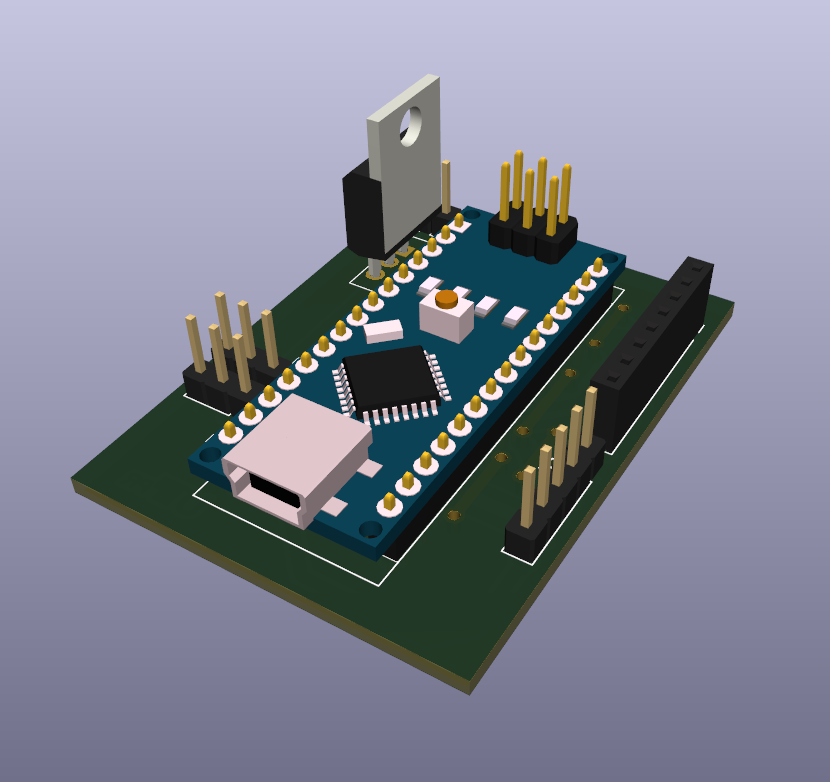
\includegraphics[width=0.6\textwidth]{Capitulo2 - Hardware/3D placa.PNG}\\
\caption{\label{fig:widgets}Modelo 3D da placa de circuito impresso.}
\end{figure}

\begin{figure}[H]
\centering
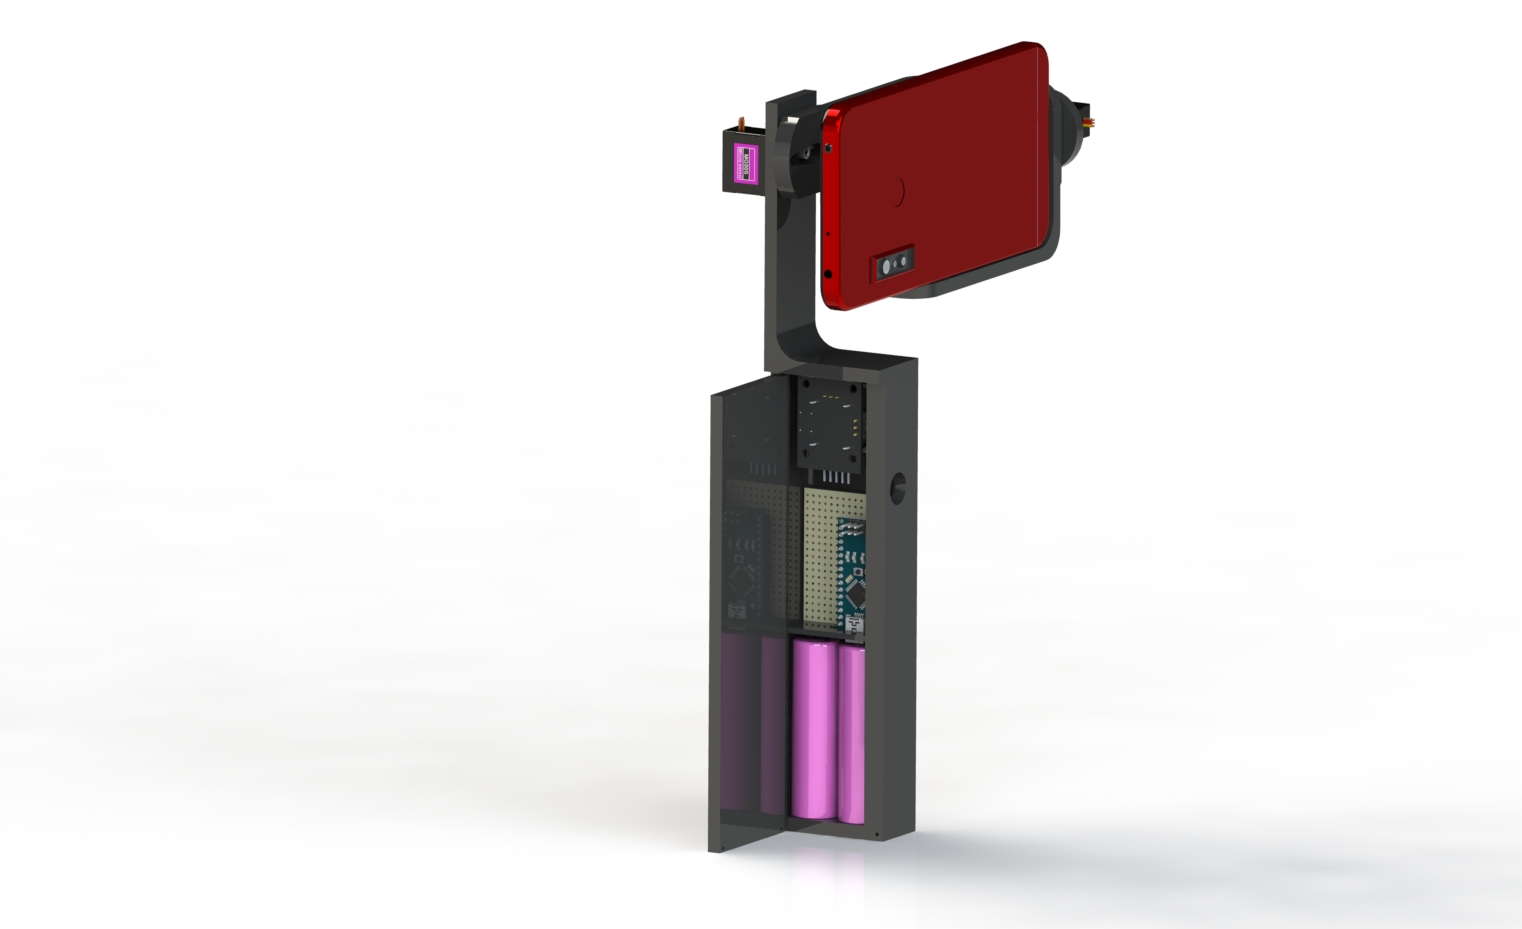
\includegraphics[width=0.6\textwidth]{Capitulo2 - Hardware/versao final.JPG}\\
\caption{\label{fig:widgets}Modelo 3D do dispositivo.}
\end{figure}


\section{Suporte articulado}
A estabilização para o equipamento preso à estrutura articulada é dada por dois eixos de rotação, estes possibilitam variar a inclinação do suporte na vertical e na horizontal de zero a 90 graus para cada lado, isto devido a cada servo motor MG90s possibilitar uma rotação de 180 graus. Cada servo motor opera entre 4,8 e 6 volts, com seu torque e velocidade de operação variando de acordo com esses parâmetros. Para um funcionamento estável, os motores não são alimentados pelo arduino, a tensão máxima fornecida aos dois servos é de 5 volts, como a tensão de saída do conjunto de baterias é de 7,2 volts, foi utilizado um regulador de tensão LM7805, que mantém uma tensão estável de 5 volts se a tensão de entrada for maior que 7 volts, não excedendo 30 volts, isso nos dá os parâmetros da tabela 2.

\begin{table}[H]
\centering
\begin{tabular}{j|j|j}
Tensão de entrada & Torque & Velocidade de operação \\\hline
4,8 & 1,8kg/cm & 0.1sec/60 graus\\
5,0 & 1,9kg/cm & 0.1sec/60 graus\\
6,0 & 2,2kg/cm & 0.08sec/60 graus\\
\end{tabular}
\caption{\label{tab:widgets}Tabela de parâmetros do servo motor MG90s para diferentes tensões de entrada.}
\end{table}

Ambos os servos são fixados diretamente na estrutura impressa por meio de dois parafusos, e as peças móveis da estrutura articulada são encaixadas diretamente no eixo de cada um dos servos com o auxilio de hélices de plástico. Para facilitar a movimentação das partes móveis e diminuir o atrito, e por consequência o desgaste do material plástico, foi adicionado sob cada eixo (encontro de duas partes móveis) duas arruelas de ferro com graxa. O cabeamento dos dois servos segue presa às estruturas móveis da estrutura articulada, isso devido ao comprimento necessário dos cabos ser diferente para diferentes posições de operação.


\section{Eletrônica}
%incluir esquematico, diagrama de blocos
O sistema conta com duas células (baterias) recarregáveis de 3,6 volts e 3000 mAh ligadas em série, fornecendo ao sistema 7,2 volts, este conjunto de baterias é ligado a um interruptor, e este é ligado à placa de circuitos. A trilha positiva se liga ao regulador de tensão LM7805 (que manda cerca de 5,0 volts aos dois servo motores), e também ao arduino nano (este não precisa de um regulador de tensão externo, como no caso dos dois servos, pois já possui um integrado em sua placa). O joystick analógico e o sensor MPU-6050 são conectados exclusivamente ao arduino conforme pode ser visto na figura 3. Todos os componentes são conectados por meio de barramentos soldados na placa, permitindo o funcionamento como pode ser visto na figura 4, dando ao sistema modularidade, uma vez que cada componente pode ser removido individualmente, facilitando operações como manutenção e ajustes.

\begin{figure}[H]
\centering
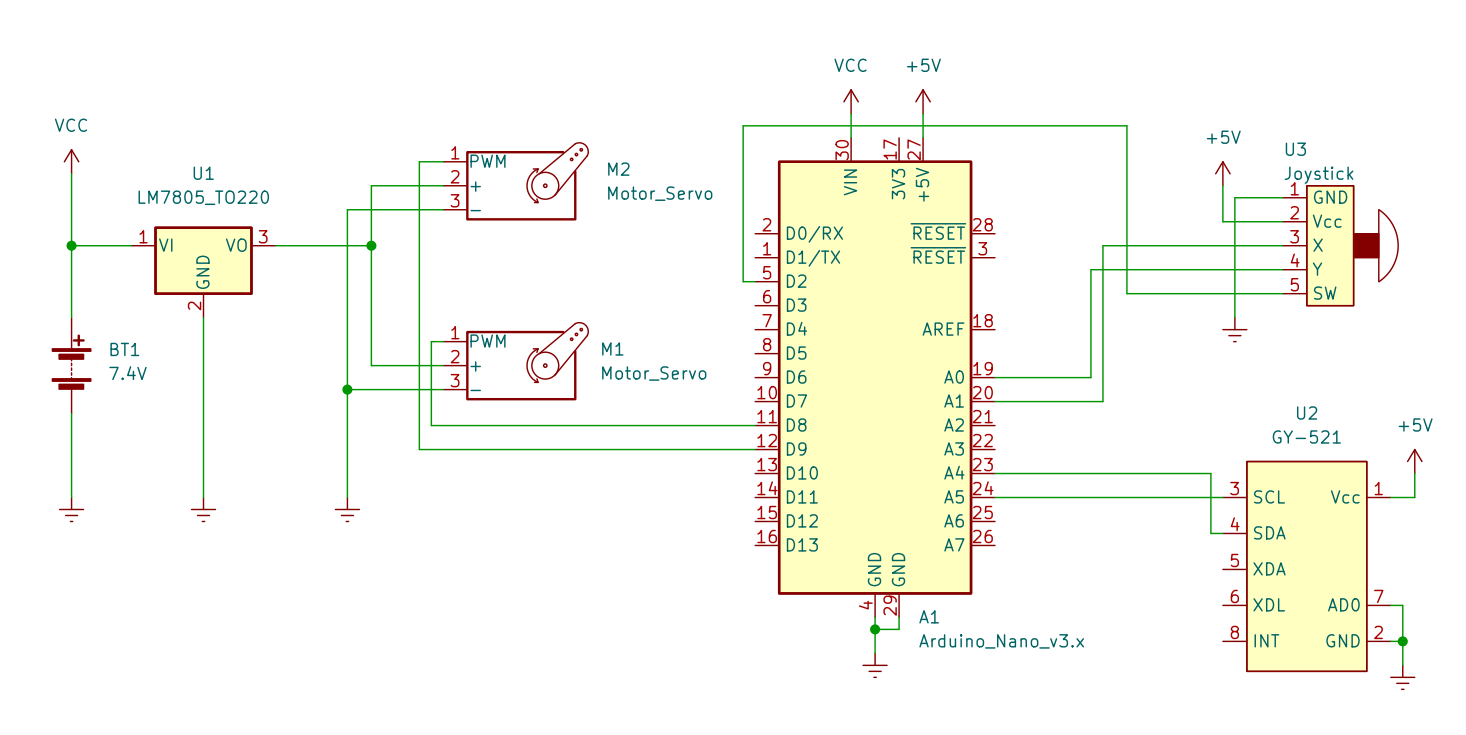
\includegraphics[width=0.9\textwidth]{Capitulo2 - Hardware/Esquematico.PNG}\\
\caption{\label{fig:widgets}Esquemático dos componentes eletrônicos.}
\end{figure}

\begin{figure}[H]
\centering
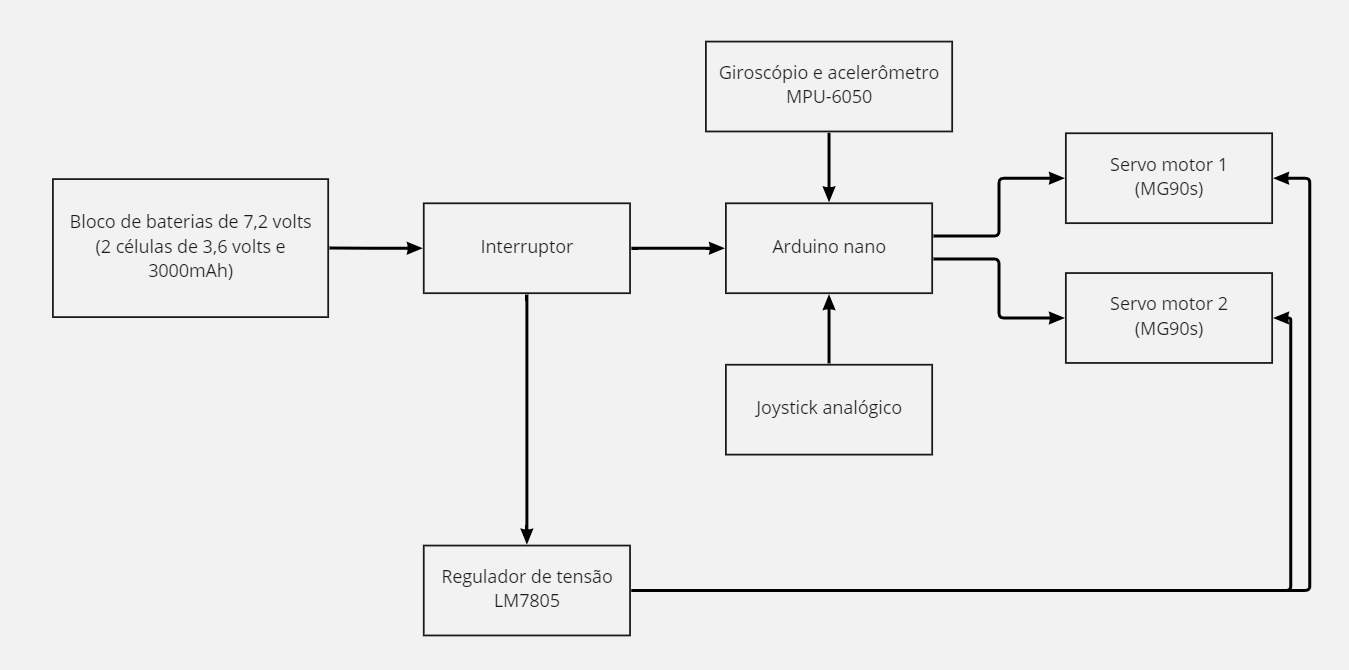
\includegraphics[width=0.9\textwidth]{Capitulo2 - Hardware/DiagramaDeBlocos.png}\\
\caption{\label{fig:widgets}Diagrama de blocos do dispositivo.}
\end{figure}


A placa de circuitos foi produzida manualmente pelos integrantes do grupo deste trabalho utilizando percloreto de ferro. A imagem do circuito foi produzida através do software KiCad, como pode ser visto na figura 5, e foi transferida de um papel fotográfico para a placa de fenolite utilizando uma fonte de calor, depois de resfriada, foi imersa em percloreto de ferro por cerca de cinco minutos. Após o fim do processo, obtivemos uma placa funcional do circuito do projeto, como pode ser visto na figura 6.

\begin{figure}[H]
\centering
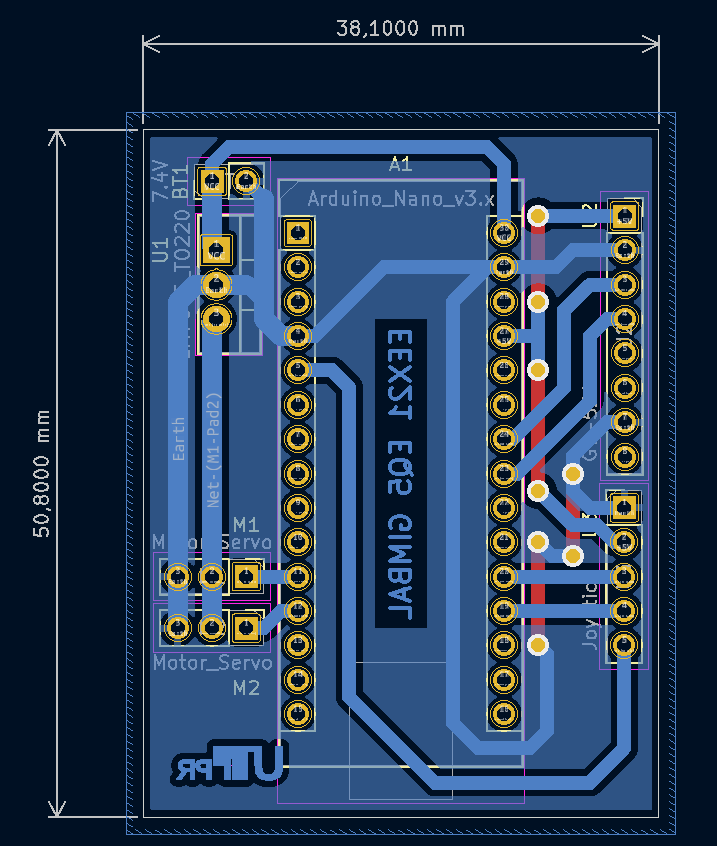
\includegraphics[width=0.5\textwidth]{Capitulo2 - Hardware/Circuito placa desenho.PNG}\\
\caption{\label{fig:widgets}Desenho do circuito no software KiCad.}
\end{figure}

\begin{figure}[H]
\centering
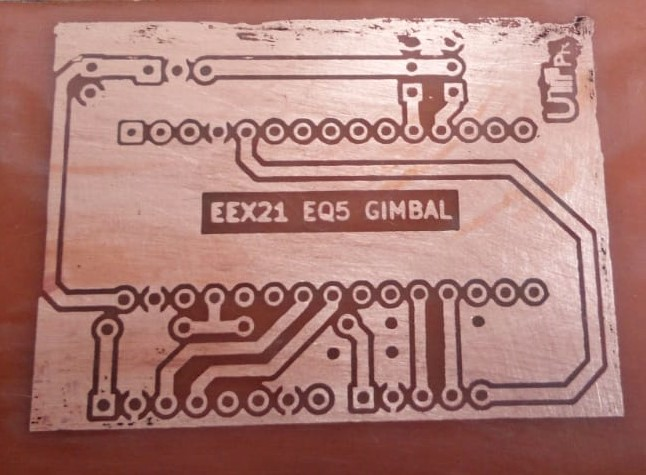
\includegraphics[width=0.5\textwidth]{Capitulo2 - Hardware/CircuitoPlaca.jpeg}\\
\caption{\label{fig:widgets}Placa produzida manualmente utilizando o processo de corrosão por percloreto de ferro.}
\end{figure}

Com exceção dos servo motores, os componentes são posicionados dentro da estrutura impressa (caixa) através de pequenos parafusos, dando espaço ao posicionamento do módulo MPU-6050 com sua placa orientada na horizontal, nos permitindo obter leituras precisas da inclinação nos dois eixos de rotação da estrutura articulada, como também possibilitar a passagem dos cabos sem prejudicar outros componentes. %% Comente para remover este item

%% Capítulo
%%%% CAPÍTULO 3 - MATERIAL E MÉTODOS (PODE SER OUTRO TÍTULO DE ACORDO COM O TRABALHO REALIZADO)
%%
%% Deve apresentar o modelo utilizado, a modelagem
%% empregada, as simplificações necessárias, a
%% metodologia e a descrição do método de cálculo 
%% utilizado no desenvolvimento da pesquisa para que
%% a mesma possa ser reconstituída. Deve ainda 
%% apresentar resultados de amostras e comentários.
%% Deve apresentar a descrição da montagem 
%% experimental, metodologia para a obtenção de 
%% resultados, análise de erros, amostra de resultados
%% obtidos e comentários. Atenção: Esta parte pode ser
%% subdividida em mais capítulos de acordo com a 
%% especificidade do assunto.

%% Título e rótulo de capítulo (rótulos não devem conter caracteres especiais, acentuados ou cedilha)
\chapter{Software}\label{cap:materialemetodos}

\section{Ferramentas e Bibliotecas}
O código do controlador foi feito utilizando o IDE do arduino e as bibliotecas "MPU6050\textunderscore light" e "Servo", disponíveis para download pelo IDE. A primeira biblioteca realiza a leitura dos sensores acelerômetro e giroscópio pelo barramento I2C do arduino, além de combiná-los com um filtro complementar que será explicado a seguir. A segunda biblioteca realiza o controle das posições dos servo motores por meio de um sinal PWM. Uma visão geral do funcionamento do sistema é dada pelo fluxograma na figura 7.

\begin{figure}[H]
\centering
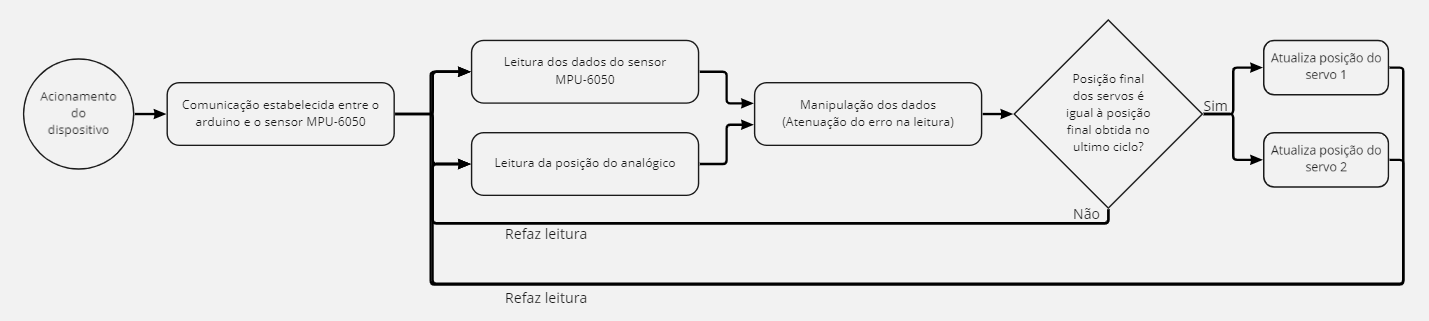
\includegraphics[width=1\textwidth]{Capitulo3 - Software/Fluxograma.png}\\
\caption{\label{fig:widgets}Fluxograma da sequencia de operação do sistema.}
\end{figure}

\section{Ângulos a partir das leituras do MPU-6050}
A leitura dos sensores é realizada pela biblioteca "MPU6050\textunderscore light", são lidos utilizando o protocolo I2C os valores brutos da aceleração linear, do acelerômetro, e angular, do giroscópio.\\
\indent Em funcionamento normal a maior aceleração linear percebida pelo dispositivo é a gravidade e, com um pouco de trigonometria, é calculada a rotação do sistema em relação à direção "para baixo". Ao longo do tempo o valor médio calculado se mantém próximo do esperado, porém qualquer movimento, até mesmo as vibrações de origem térmica no material, causam ruídos e ainda não podemos utilizar essa leitura diretamente.\\
\indent Das leituras da aceleração angular podemos integrar o sinal duas vezes para obter a velocidade angular e então o ângulo relativo à alguma posição de referência. Para um tempo curto essa leitura já basta, contudo o erro do sistema é somado em cada ciclo de integração e um desvio vai se acumulando com o tempo. Outro problema que precisa ser corrigido antes de utilizar essa leitura é a definição dessa posição de referência.\\
\\
\indent Pode-se observar então que temos uma variável com boa confiança em curto prazo (do giroscópio) e outra cuja a confiança é aceitável apenas após a coleta de várias leituras após um longo tempo para ser calculada uma média (do acelerômetro). Pode-se então utilizar a técnica de filtros complementares para combinar o sinal dos dois sensores e ter o melhor dos dois mundos. A figura 8 apresenta um diagrama em blocos do filtro implementado pela biblioteca. O parâmetro k controla qual medição vai ter mais influência em curto prazo e, por complemento, qual teria mais influência após um tempo muito longo. Valores típicos são cerca 99\%, dando um peso maior para as leituras de ângulo pelo giroscópio em curto prazo e para o acelerômetro, que vai fazer o trabalho da posição de referência, após muito tempo.

\begin{figure}[H]
\centering
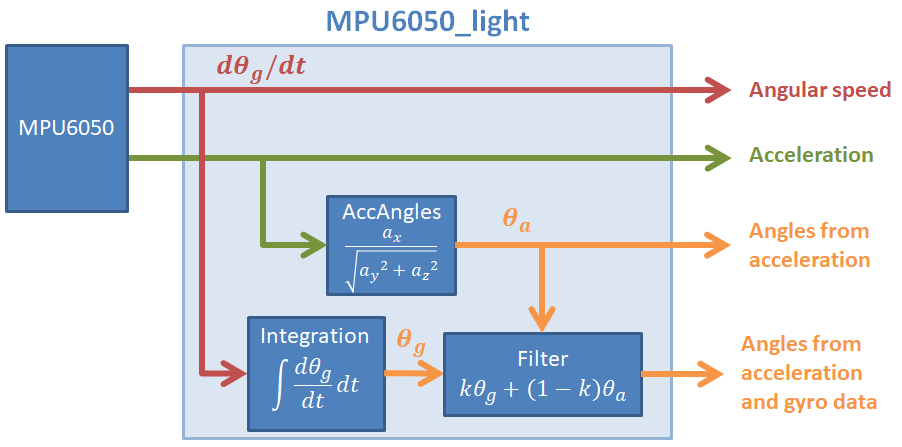
\includegraphics[width=1\textwidth]{Capitulo3 - Software/FiltroComplementar.png}\\
\caption{\label{fig:widgets}Operação do filtro - Imagem obtida na documentação da biblioteca "MPU6050\textunderscore light"}
\end{figure}

\section{Testes sem a estrutura 3D}

Durante o desenvolvimento do projeto foi utilizada uma aplicação web 3d para testes com sensor MPU-6050, que nos permitiu analisar seu funcionamento sem ter de acoplar motores ou quaisquer outros atuadores, tal aplicação é executada no navegador Chrome ou semelhante do computador, sendo necessário somente que o sensor esteja ligado a um arduino, e este arduino, ligado ao computador. Ao iniciar a aplicação, é solicitada a porta serial conectada ao sistema com o sensor, com isso, a interface fornece um cubo, como mostrado na figura 9, que acompanha a rotação do sensor no mundo real.

\begin{figure}[H]
\centering
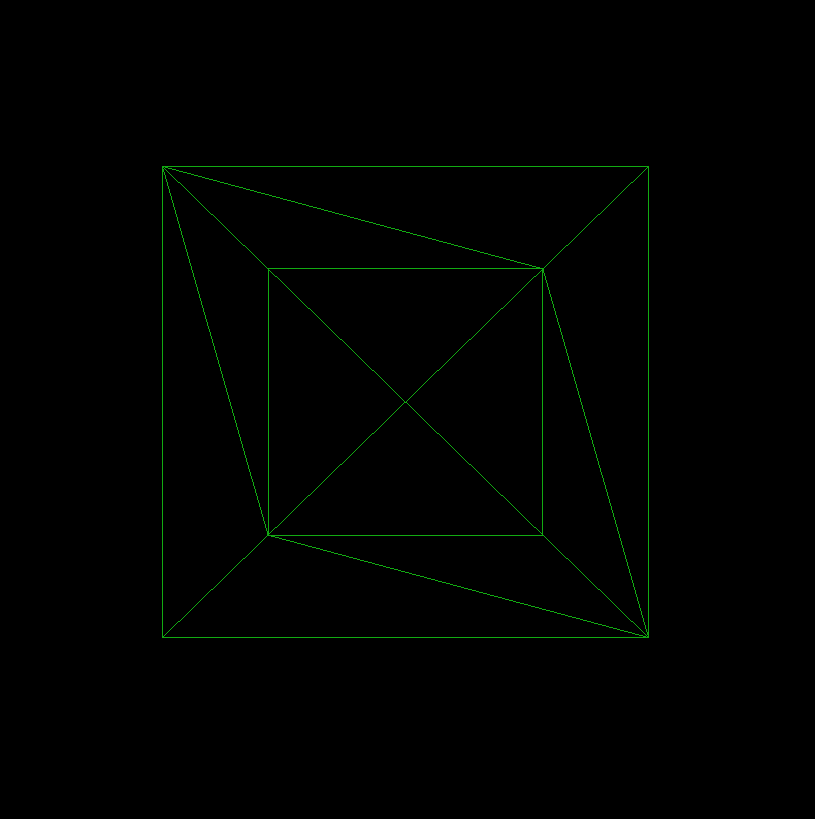
\includegraphics[width=0.6\textwidth]{Capitulo3 - Software/3dcubo.png}\\
\caption{\label{fig:widgets}Fluxograma da sequencia de operação do sistema.}
\end{figure}

\section{Leitura do Joystick}
No joystick é feito três leituras, o eixo x, eixo y e um botão de reset. Os eixos de movimento são lidos direto por portas analógicas no arduino e o botão por uma porta digital.\\
\indent O joystick controla um ajuste para cada eixo, esses ajustes são dois ângulos de desvio a ser considerados no posicionamento dos motores. Movendo um eixo do joystick para uma posição positiva o ajuste correspondente é incrementado com o tempo. O simétrico vale para uma posição negativa também. Podemos imaginar um plano "Ajuste X x Ajuste Y" com um ponto cujas as coordenadas são um ajuste final, o joystick então movimentaria esse ponto como se fosse um personagem de um jogo.

\pagebreak
\section{Controle dos servomotores}

Os servomotores são controlados por um sinal modulado por largura de pulso (PWM). O período do sinal é de 20ms e a largura de pulso varia entre 1ms e 2ms, que posicionam o servo nas posições 0º e 180º, respectivamente. Para poupar tempo de desenvolvimento foi utilizada a biblioteca "Servo" que gera essas formas de onda.\\
\indent Da saída do filtro complementar já temos um bom posicionamento, mas ainda causa solavancos extremos em quase todo movimento. Antes de enviar a nova posição de correção para os servos esse sinal ainda é tratado com um filtro de média levando em conta os últimos 5 valores e é adicionado o valor de ajuste do joystick. Então a posição do servomotor é interpolada entre a posição antiga e a nova posição corrigida. Dessa forma no começo de uma correção os motores se movimentam rapidamente e conforme se aproximam da posição final eles desaceleram, reduzindo os solavancos.%% Comente para remover este item

%% Capítulo
%%%% CAPÍTULO 4 - RESULTADOS E DISCUSSÃO
%%
%% Deve descrever detalhadamente os dados obtidos 
%% pelo autor. Normalmente são incluídas ilustrações
%% como: quadros, tabelas, gráficos, etc. Deve efetuar
%% a comparação dos dados obtidos e/ou resultados, com
%% aqueles descritos na revisão de literatura, 
%% incluindo os comentários sobre os estudos de outros
%% autores.

%% Título e rótulo de capítulo (rótulos não devem conter caracteres especiais, acentuados ou cedilha)
\chapter{Resultados}\label{cap:resultadosediscussao}

\section{Hardware}
Os resultados obtidos com o protótipo do dispositivo evidenciaram que, para grandes vibrações, o dispositivo funciona como esperado, anulando as inclinações indesejadas e mantendo a estrutura articulada estável, o qual, junto dos sistemas de estabilização embutidos no equipamento de vídeo, fornece uma imagem com poucas vibrações, oque já era esperado, uma vez que o sistema estabiliza o suporte articulado dentro de limites de operação.\\
\\
\indent Foi observado que, movimentos bruscos de "grande amplitude" podem gerar leituras fora dos padrões pelo sensor MPU-6050, com a grande maioria destas anormalidades sendo anulada via software, porém, isso não se mostrou um problema, uma vez que o propósito de um estabilizador externo é amenizar vibrações (como vibrações encontradas em um caminhar, durante a gravação de um show ou outros eventos artísticos) e não balancear movimentos demasiadamente grandes, que inclinem o equipamento mais que 90 graus para qualquer um dos lados ou movimentos súbitos (como chacoalhar o equipamento ou coloca-lo de cabeça para baixo).

\section{Software}
Foi observado durante o desenvolvimento do projeto, dificuldade na integração das leituras dadas pelo sensor MPU-6050 com os servo motores, posteriormente concluímos que o problema quanto a rotação dos servos era a falta de um "filtro" para os valores obtidos pelo sensor, a falta deste filtro ocasionava na tentativa de correção de orientação da estrutura articulada a cada pequena variação na leitura do sensor, este, por possuir erro constante na leitura de cerca de 1 grau positivo ou negativo e uma nova leitura acontecendo a cada 20 milissegundos, ocasionava a instabilidade de toda a estrutura articulada.

\section{Design final}
O design final do dispositivo pode ser visto nas figuras 10 e 11.


\begin{figure}[H]
\centering
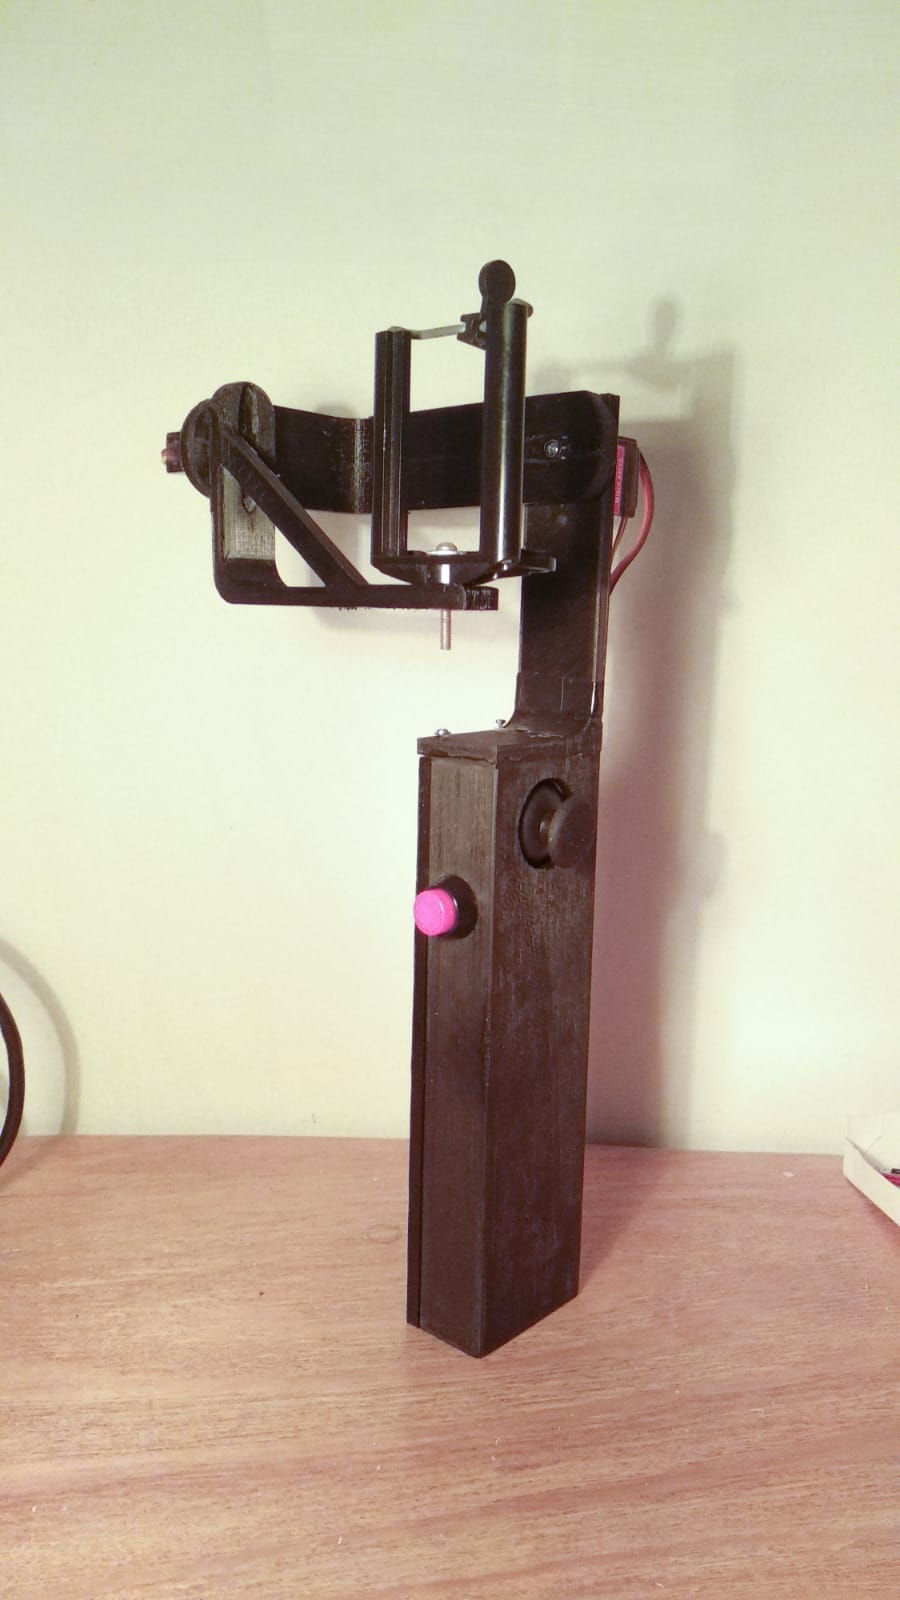
\includegraphics[width=0.4\textwidth]{Capitulo4 - Resultados/dir.jpeg}\\
\caption{\label{fig:widgets}Design final do dispositivo.}
\end{figure}

\begin{figure}[H]
\centering
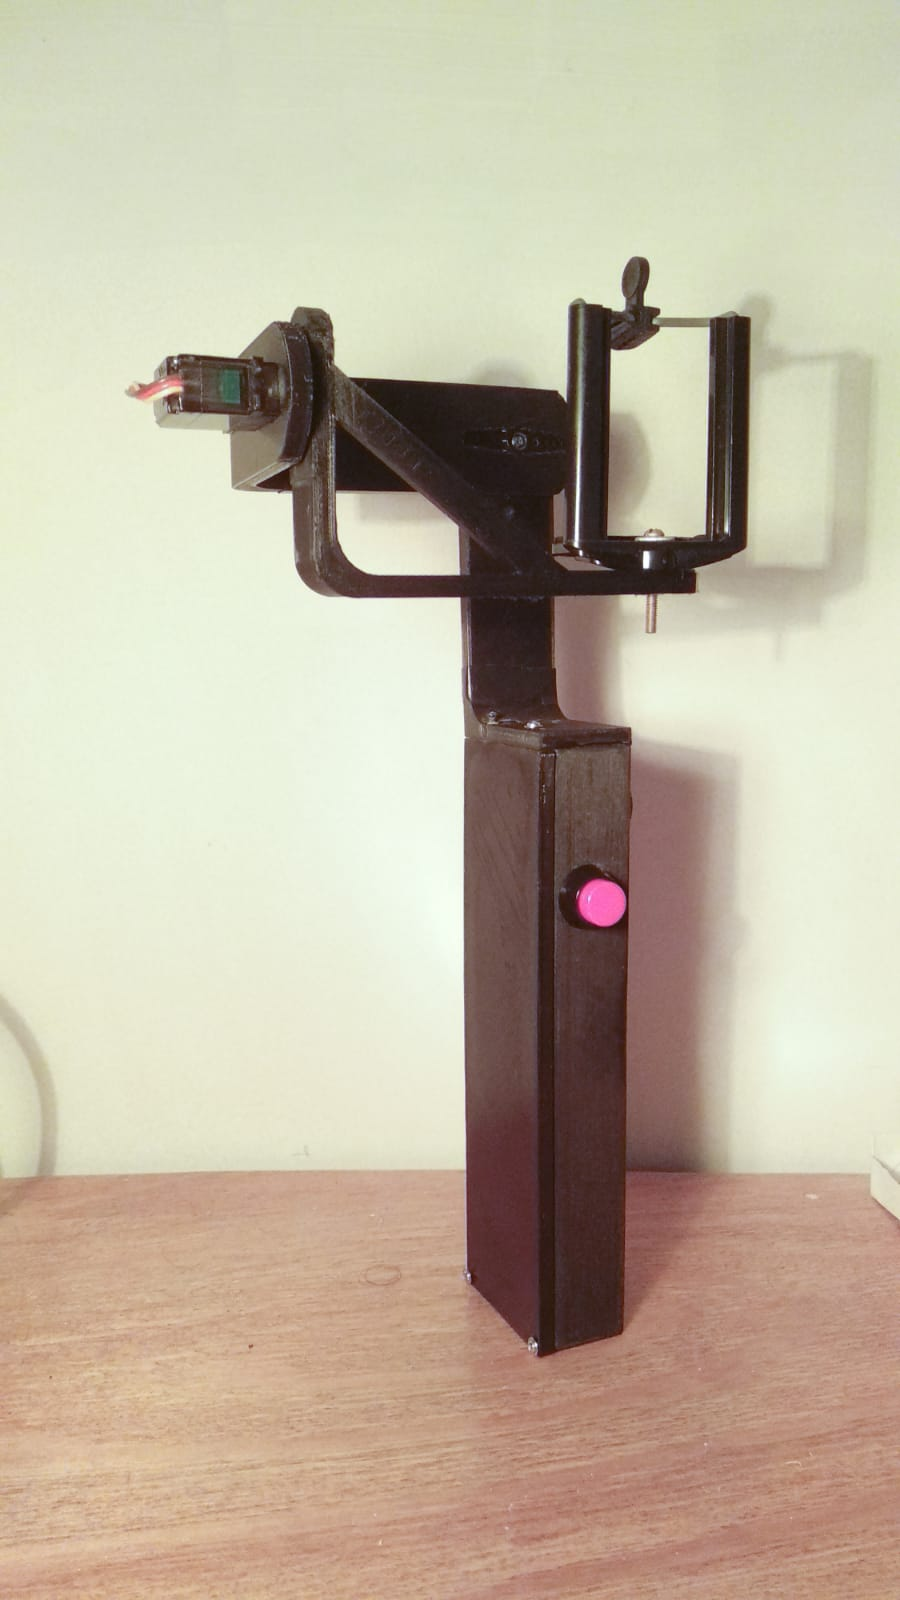
\includegraphics[width=0.4\textwidth]{Capitulo4 - Resultados/esq.jpeg}\\
\caption{\label{fig:widgets}Design final do dispositivo.}
\end{figure}%% Comente para remover este item

%% Parte
%\part{Conclusão}%% Comente para remover este item

%% Capítulo
%%%% CAPÍTULO 5 - CONCLUSÕES E PERSPECTIVAS
%%
%% Deve finalizar o trabalho com uma resposta às
%% hipóteses especificadas na introdução. O autor deve
%% manifestar seu ponto de vista sobre os resultados
%% obtidos; não se deve incluir neste capítulo novos
%% dados ou equações. A partir da tese, alguns assuntos
%% que foram identificados como importantes para serem
%% explorados poderão ser sugeridos como temas para
%% novas pesquisas.

%% Título e rótulo de capítulo (rótulos não devem conter caracteres especiais, acentuados ou cedilha)
\chapter{Conclusões}\label{cap:conclusoeseperspectivas}

Apesar das dificuldades encontradas durante a construção e programação do dispositivo, nota-se que, mesmo componentes de prototipação conseguem entregar um resultado aceitável. Este projeto, mesmo sendo conceitualmente simples, se mostrou desafiador devido a possuir partes móveis acopladas, oque a principio, gerou problemas de estabilidade e, no caso da estrutura articulada, retrabalho de algumas peças. Além disso, o uso de ferramentas de edição 3d facilitou muito o trabalho de construí-lo, assim como a visualização 3d das leituras do sensor por meio de um software contribuiu para o entendimento do funcionamento do mesmo.
%% Comente para remover este item

\chapter{Referencias}

\phantom{aaa}\\
Repositório de arquivos do projeto. Disponível em <https://github.com/ratatusznei/gimbal-EEX21> Acessado durante todo o período de desenvolvimento do projeto.\\\\
Biblioteca MPU6050\textunderscore light. Disponível em <https://github.com/rfetick/MPU6050\textunderscore light> Acessado durante todo o período de desenvolvimento do projeto.\\\\
Vídeo do projeto, ESTABILIZADOR DE DOIS EIXOS PARA CÂMERAS. Disponível em <https://youtu.be/y9m5s8JzXt0>

%% Capítulos após este comando criam marcadores do pdf na raiz
% \phantompart%% Comente para remover este item

%% Capítulo de exemplo
%\include{./CapituloExemplo/capituloexemplo}%% Comente para remover este item


%%%%%%%%%%%%%%%%%%%%%%%%%%%%%%%%%%%%%%%%%%%%%%%
%%%%%%%%%%%%%%%%%%%%%%%%%%%%%%%%%%%%%%%%%%%%%%%
%% Formatação de páginas de elementos pós-textuais
%%
\postextual%% Não comente esta linha


%%%%%%%%%%%%%%%%%%%%%%%%%%%%%%%%%%%%%%%%%%%%%%%
%% Arquivos de referências
%%
\arquivosdereferencias{%% Arquivos bibtex sem a extensão .bib e separados por vírgula - Não comente esta linha
  %./PosTexto/exemplos-referencias,%% Arquivo de referências - Comente para remover este item (chktex 26 supress warn.)
  %./PosTexto/referencias%% Arquivo de referências - Comente para remover este item (chktex 26 - supress warn.)
}%% Não comente esta linha
%%%%%%%%%%%%%%%%%%%%%%%%%%%%%%%%%%%%%%%%%%%%%%%


%% Fim do documento
\end{document}%% Não comente esta linha
%%%%%%%%%%%%%%%%%%%%%%%%%%%%%%%%%%%%%%%%%%%%%%%